%%%%%%%%%%%%%%%%%%%%%%%%%%%%%%%%%%%%%%%%%
% University/School Laboratory Report
% LaTeX Template
% Version 3.1 (25/3/14)
%
% This template has been downloaded from:
% http://www.LaTeXTemplates.com
%
% Original author:
% Linux and Unix Users Group at Virginia Tech Wiki 
% (https://vtluug.org/wiki/Example_LaTeX_chem_lab_report)
%
% License:
% CC BY-NC-SA 3.0 (http://creativecommons.org/licenses/by-nc-sa/3.0/)
%
%%%%%%%%%%%%%%%%%%%%%%%%%%%%%%%%%%%%%%%%%

%----------------------------------------------------------------------------------------
%	PACKAGES AND DOCUMENT CONFIGURATIONS
%----------------------------------------------------------------------------------------

\documentclass[UTF8]{ctexart}

\usepackage{siunitx} % Provides the \SI{}{} and \si{} command for typesetting SI units
\usepackage{graphicx} % Required for the inclusion of images
\usepackage{subfigure}
\usepackage{natbib} % Required to change bibliography style to APA
\usepackage{amsmath} % Required for some math elements 
\usepackage{amssymb} % 使用因为所以符号
\usepackage{fancyhdr} % 使用页眉

\usepackage{algorithm}
\usepackage{algorithmic}

\pagestyle{fancy}
\fancyhf{} 
\cfoot{\thepage} 
% TODO 自定义页眉
% TODO 解释python不会溢出的原因

\setlength\parindent{0pt} % Removes all indentation from paragraphs

\renewcommand{\labelenumi}{\alph{enumi}.} 

%----------------------------------------------------------------------------------------
%	DOCUMENT INFORMATION
%----------------------------------------------------------------------------------------
\title{算法分析与设计-作业二}

\author{王宸昊 2019214541}

\date{\today}

\begin{document}

\maketitle

%----------------------------------------------------------------------------------------
%	SECTION 1
%----------------------------------------------------------------------------------------

\section{最近点对}

% If you have more than one objective, uncomment the below:
%\begin{description}
%\item[First Objective] \hfill \\
%Objective 1 text
%\item[Second Objective] \hfill \\
%Objective 2 text
%\end{description}

\subsection{算法简介}

\begin{description}
\item[Stoichiometry]
The relationship between the relative quantities of substances taking part in a reaction or forming a compound, typically a ratio of whole integers.
\item[Atomic mass]
The mass of an atom of a chemical element expressed in atomic mass units. It is approximately equivalent to the number of protons and neutrons in the atom (the mass number) or to the average number allowing for the relative abundances of different isotopes. 
\end{description} 

\subsection{算法伪代码}

\subsection{实验效果}

\subsection{进一步改进}

\subsection{界面展示}

%----------------------------------------------------------------------------------------
%	SECTION 2
%----------------------------------------------------------------------------------------
\section{三种不同的方法求Fibonacci数}

\subsection{算法简介}
斐波那契数列(Fibonacci Sequence)是指1,1,2,3,5,8$\dots$这样的数列,在数学上使用一下递推的方式定义:

\begin{equation*}
    f(n) =
    \begin{cases}
    0, & \mbox{if }n\mbox{ = 0} \\
    1, & \mbox{if }n\mbox{ = 1} \\
    F(n)=F(n-1)+F(n-2), & \mbox{if }n \geq 2
    \end{cases}    
\end{equation*}

在本次实验中,采用三种不同的算法对Fibonacci数列进行计算,分别是递归法、迭代法和矩阵法。对于不同的算法采用的策略不同,算法的运行时间和结果的精度都不尽相同,在下面的实验中,会对不同的算法的性能进行对比。

\begin{description}
\item[递归法] 递归法利用分治的思想,将规模为n问题分解为n-1和n-2规模的问题,借助自身函数调用解决问题。但是递归法也存在着很多的问题,例如递归调用栈不能太深,否则程序无法正常运行;递归法中存在着大量重复的计算,极大影响了算法执行的效率。
\item[迭代法]
迭代法的算法思想更加直观,不断利用前两个元素的值累加迭代得到下一个结果,与递归法相比,减少了很多重复的计算,而且计算的复杂度也是线性的。
\item[矩阵法]
矩阵法是利用了分治算法的思想,将求解斐波那契数列的问题转化为等价的矩阵运算,利用分治法的算法思想,将矩阵运算分解为规模更小的问题进行求解。其算法复杂度为$lg(n)$,在实际的实验中,其算法的执行时间比较优秀,但是由于涉及到矩阵乘法,存在着算数精度的问题。
\end{description} 

\subsection{算法伪代码}

递归法:
\begin{algorithm}[H]
	\caption{FIB\_RECUR$(n)$}%算法标题
    \begin{algorithmic}[1]%一行一个标行号
        \IF{$n\leq1$}
        \RETURN{n}
        \ENDIF
        \RETURN{FIB\_RECUR(n-1) + FIB\_RECUR(n-2)}
	\end{algorithmic}
\end{algorithm}

迭代法:
\begin{algorithm}[H]
	\caption{FIB\_LOOP$(n)$}%算法标题
	\begin{algorithmic}[1]%一行一个标行号
        \STATE $a = 0$
        \STATE $b = 1$
		\FOR{$i=0$ to $n$}
		\STATE $a = b$
		\STATE $b = a + b$
        \ENDFOR
        \RETURN{a}
	\end{algorithmic}
\end{algorithm}

矩阵法:
\begin{algorithm}[H]
	\caption{FIB\_MATRIX$(n)$}%算法标题
	\begin{algorithmic}[1]%一行一个标行号
		\STATE $matrix = [1,1 ; 1,0]$
		\RETURN{pow(matrix, n)}
	\end{algorithmic}
\end{algorithm}


\subsection{实验效果}
首先介绍实验的实验环境。
编译环境为Python3.6,操作系统的版本为Win10。
CPU为AMD Ryzen 7 1700(3.0 GHz),RAM 8G。\\
测试环境下,使用Python中time模块进行测量算法执行时间,最高精度达到微秒级别。此外还额外使用numpy模块进行高精度矩阵运算。\\
在实验方法上,将输入规模n逐渐增大,为了降低随机因素对执行效果的影响,对于每一个n进行10次计算取平均值。\\

不同方法的算法执行时间如下:\\
递归法的结果如图(\ref{img1})所示,递归法的算法执行时间增长的速度非常快,在计算前20项时,运行时间基本在1ms以下,但是当n继续增大时,算法的执行之间明显上升,在n达到30左右,算法执行时间大约为350ms,而当n达到40时,所需的时间到达了44810ms,当n到47以后,算法再继续计算新的结果。由此可见,在递归的情况下,当递归层数达到40以上,很难计算出结果。\\

\begin{figure}[H]
    \centering
    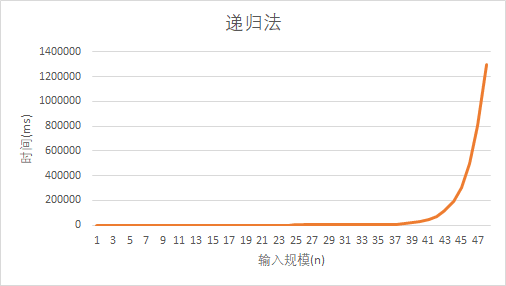
\includegraphics[width=1\textwidth]{img/1.png}
    \caption{递归法运行时间}
    \label{img1}
\end{figure}

矩阵法的结果如图(\ref{img2})所示,矩阵法的执行效果要优于递归法。虽有波动,但是整体上算法增长的速度比较慢,n在100以下的时候,基本上都在10ms以下能计算出结果。但是矩阵法存在巨大的精度问题,在Python中,int类型是不会溢出的,但是在实际的计算中,由于使用numpy的矩阵乘法,其数据长度对多支持64位,在实际的实验中可以观察到,所以当n大于93时,在计算矩阵乘法时,会产生溢出,导致得到的斐波那契数出现负数。

\begin{figure}[H]
    \centering
    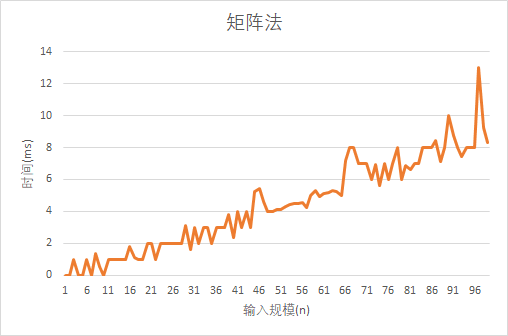
\includegraphics[width=1\textwidth]{img/2.png}
    \caption{矩阵法运行时间}
    \label{img2}
\end{figure}

迭代法的结果如图(\ref{img3})所示,综合三个算法,迭代法是最稳定的算法,在大规模的输入规模的情况下仍可以保证算法的执行时间,并且不存在溢出的问题。可以观察到,在输入规模10000的情况下,在100ms内仍可以得到结果,在实际的测试中,输入的n最多可以达到60万,结果可以在4000ms左右得到。在精度的上,由于迭代法只有加法运算,在Python中对int类型做了特殊的处理,保证在整型的情况下,不会出现溢出的情况。

\begin{figure}[H]
    \centering
    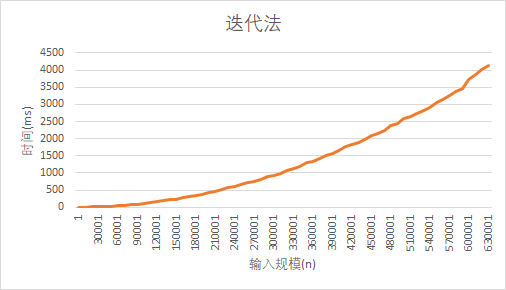
\includegraphics[width=1\textwidth]{img/3.png}
    \caption{迭代法运行时间}
    \label{img3}
\end{figure}

算法的运行时间对比如图(\ref{img4})所示。由于迭代法的输入规模明显大于其他两种方法,效果也明显优于其他两种方法,因此并没有在图上画出。从图上可以看出,蓝色线代表递归法的运行时间,对应时间刻度为左侧的坐标轴;橘色代表的是矩阵法的运行时间,对应时间刻度为右侧的坐标轴。通过对比可以看出,在相同的输入n下,递归法的运行时间比矩阵法的运行时间要高很大的数量级。

\begin{figure}[H]
    \centering
    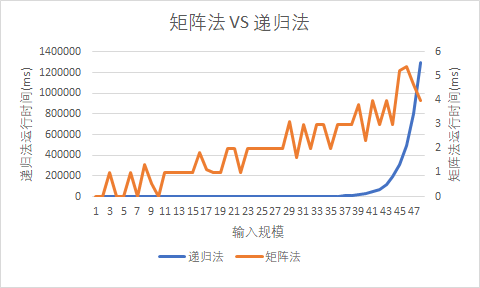
\includegraphics[width=1\textwidth]{img/4.png}
    \caption{矩阵法VS递归法}
    \label{img4}
\end{figure}

综合以上实验结果来看,迭代法效果无论从精度还是时间上,都明显优于其他两种方法。矩阵法在小规模输入下精度和执行时间也比较优秀,递归法的算法性能最差。

%----------------------------------------------------------------------------------------
%	SECTION 3
%----------------------------------------------------------------------------------------

\section{CLRS, Page, 72 5.3-4}

证明:\\
(1) 根据题意得,当dest = j 时,表示$A[i]$出现在$B[j]$的位置,即当$i+offset = j$ 或 $i+offset-n = j$。根据offset的含义可知,offset只是在原A[i]的数组的基础上循环移位offset位,对于每个i,映射到B中的唯一位置j中。$\therefore$ offset取不同值B[j]的取值不同,A[i]出现在B[j]的概为$\frac{1}{n}$ \\
(2) 此算法没有改变数组元素之间的相对位置,并不能产生均匀随机排列。\\
由上一问可知,此算法最多产生n种排列,而均匀随机排列应有n!种。\\
例如假设$A[]={[1,2,3]}$。随机排列应有$3!=6$种,根据此算法的执行过程,当offset=1时,B[]=[3,1,2];当offset=2时,B[]=[2,3,1];当offset=3时,B[]=[1,2,3]。只能得到3种排列,无法产生类似[2, 1, 3]类似的排列。

%----------------------------------------------------------------------------------------
%	SECTION 4
%----------------------------------------------------------------------------------------

\section{CLRS, Page, 73 5.3-5}

证明: \\
设$X_i$表示第i个位置元素唯一,共有$n^3$个元素。则每个位置的元素都唯一的概率为:
\begin{align*}
    P(\text{所有元素都唯一}) &= P(X_1\bigcap X_2\bigcap X_3 \cdots \bigcap X_n) \\
        &= 1(1-\frac{1}{n^3})(1-\frac{2}{n^3})(1-\frac{3}{n^3})\cdots(1-\frac{n}{n^3})\\
        &\geq 1(1-\frac{n}{n^3})(1-\frac{n}{n^3})(1-\frac{n}{n^3})\cdots(1-\frac{n}{n^3})\\
        &\geq (1-\frac{1}{n^2})^n\\
        &\geq (1-\frac{1}{n})
\end{align*}

\end{document}